\begin{tikzpicture}[scale=0.4]
    \node[above] at (16.3, 3) {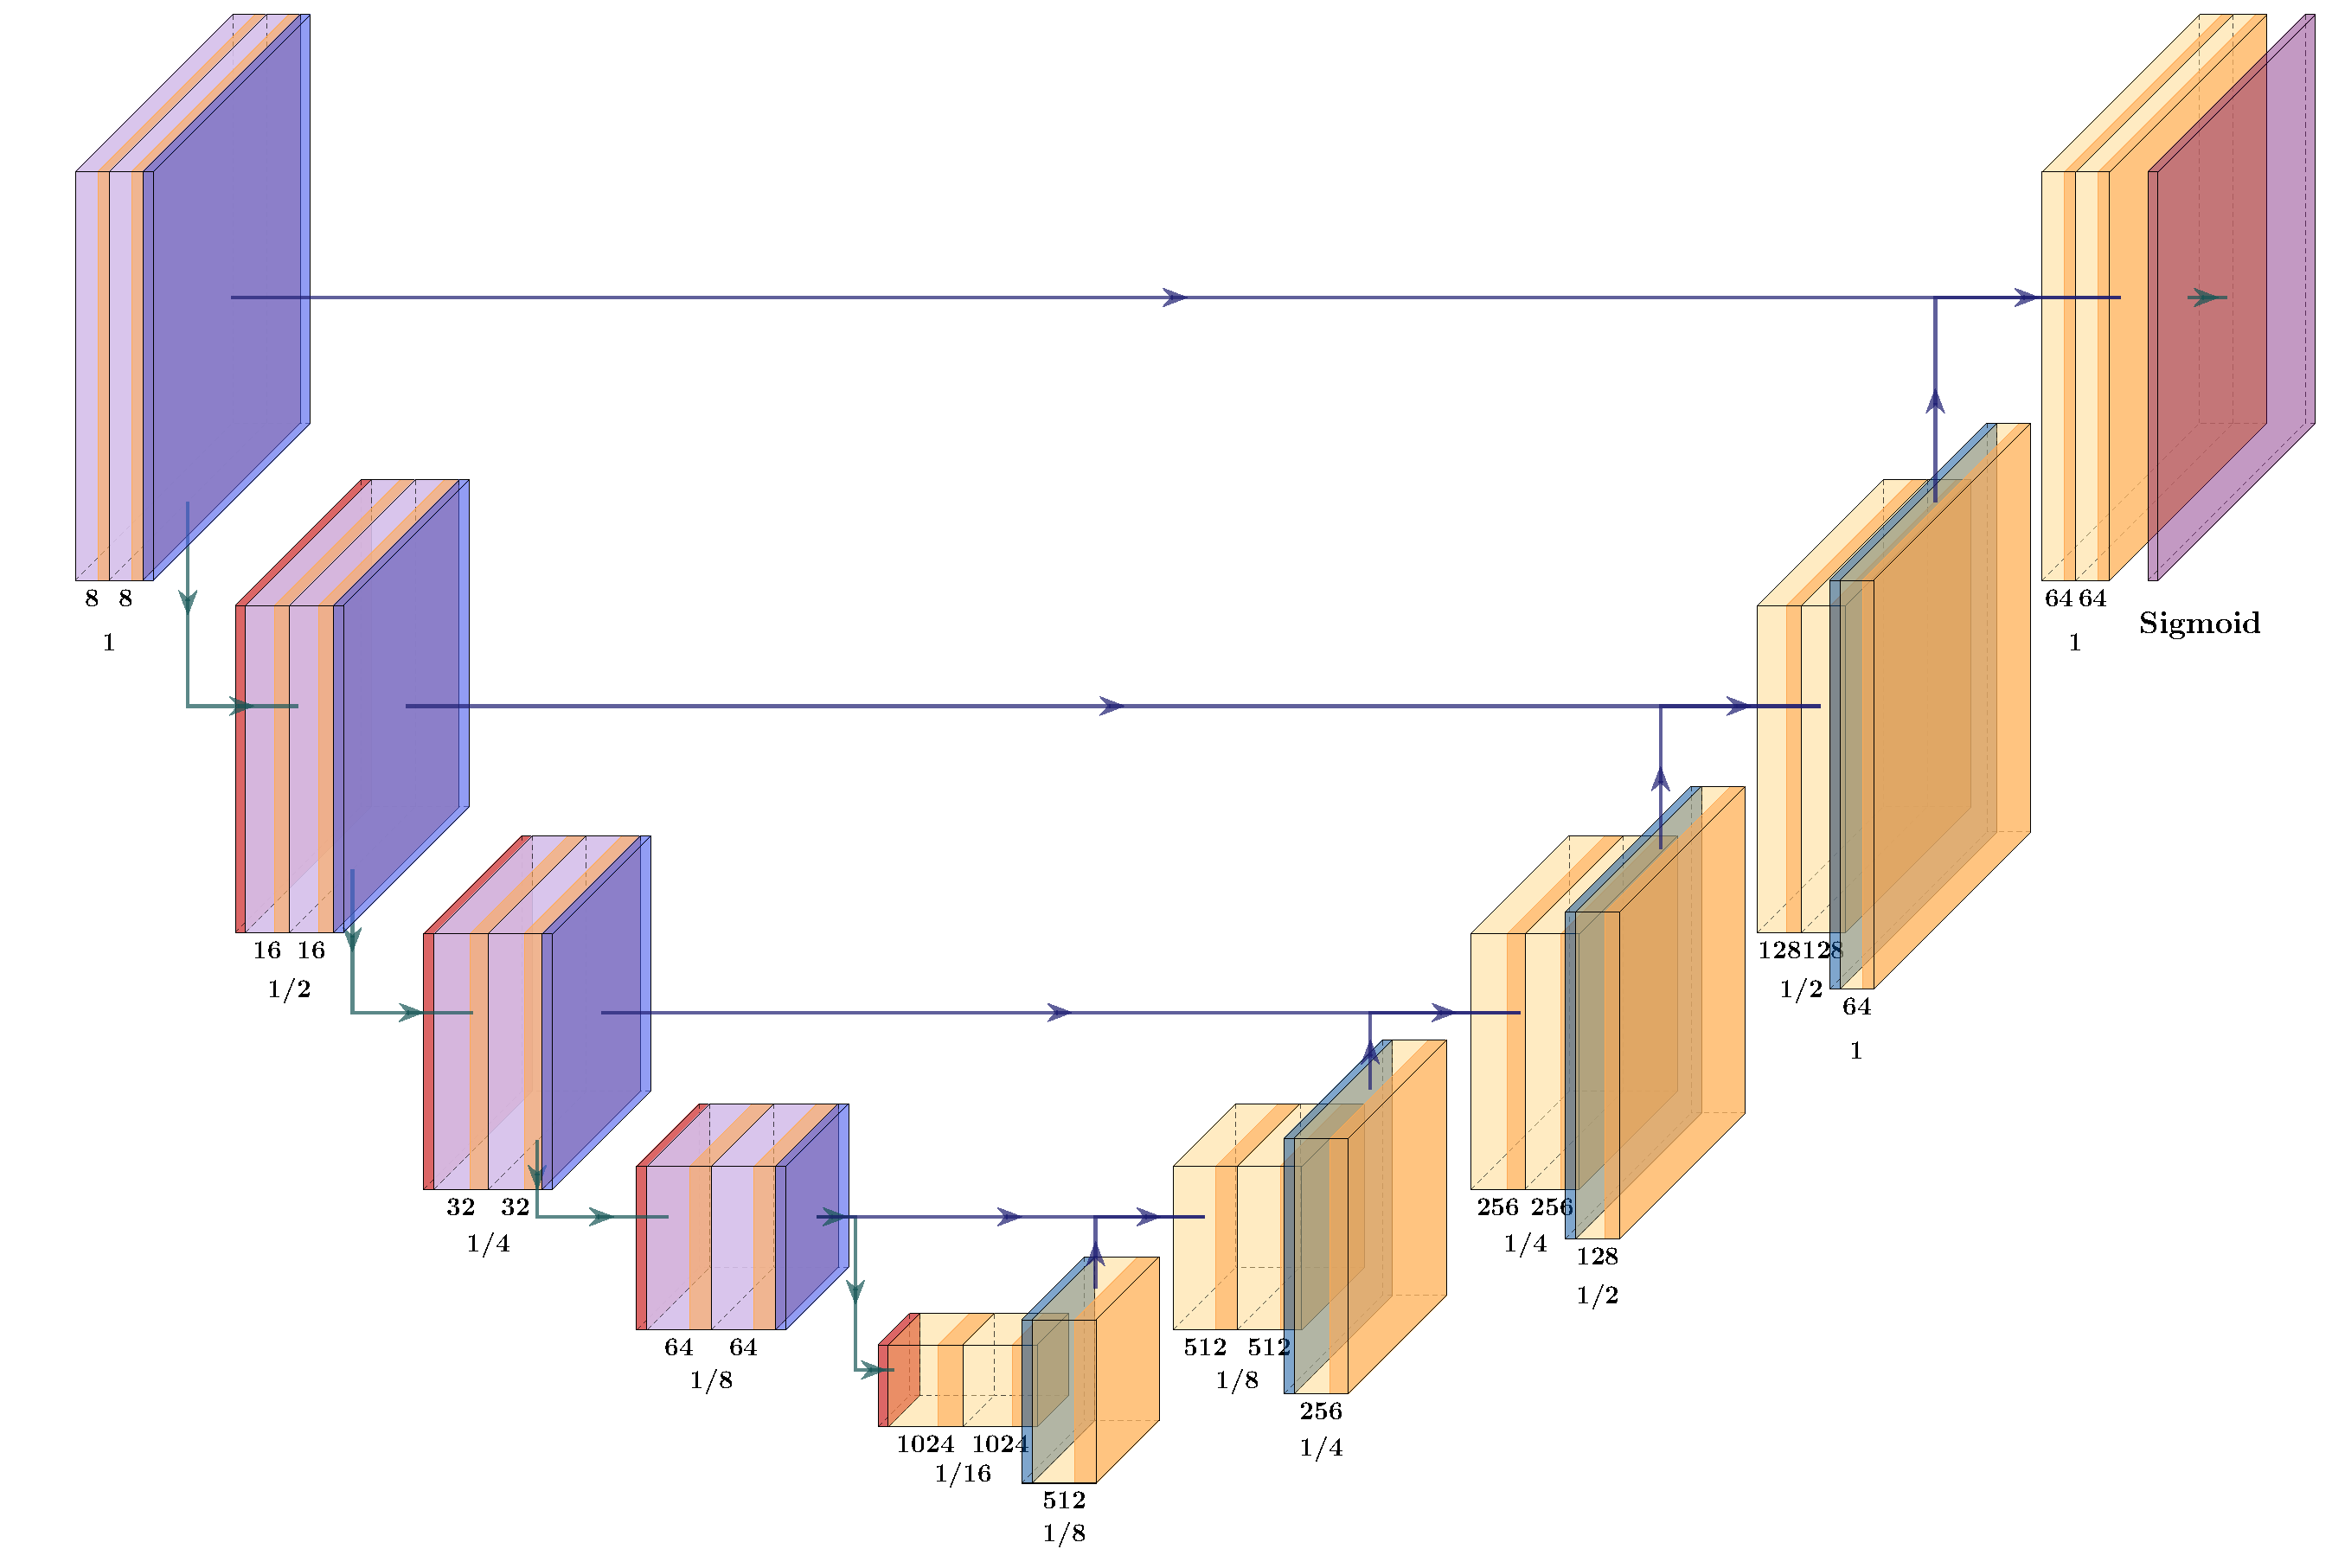
\includegraphics[width=1\textwidth]{images/U-Net-3D.pdf}};
    
    \filldraw[color=\ReshapeColor, opacity=0.7] (0,1.5) rectangle (1,2.5);
    \draw[] (0,1.5) rectangle (1,2.5);
    \node[right] at (1, 2) {\scriptsize{3$\times$3$\times$3 Convolution}};
    
    \filldraw[color=\ConvReluColor, opacity=0.8] (0,0) rectangle (1,1);
    \draw[] (0,0) rectangle (1,1);
    \node[right] at (1, 0.5) {\scriptsize{ReLU}};
    
    \filldraw[color=\ConvColorThree, opacity=0.7] (9,1.5) rectangle (10,2.5);
    \draw[] (9,1.5) rectangle (10,2.5);
    \node[right] at (10, 2) {\scriptsize{3D to 2D reshape}};
    
    \filldraw[color=\ConvColor, opacity=0.5] (9,0) rectangle (10,1);
    \draw[] (9,0) rectangle (10,1);
    \node[right] at (10, 0.5) {\scriptsize{3$\times$3 Convolution}};
    
    \filldraw[color=\PoolColor, opacity=0.6] (18,0) rectangle (19,1);
    \draw[] (18,0) rectangle (19,1);
    \node[right] at (19, 0.5) {\scriptsize{1$\times$2$\times$2 Max-pooling}};
    
    \filldraw[color=\UnpoolColor, opacity=0.5] (18,1.5) rectangle (19,2.5);
    \draw[] (18,1.5) rectangle (19,2.5);
    \node[right] at (19, 2) {\scriptsize{2$\times$2 Up-convolution}};
    
    % \filldraw[color=\PoolColor, opacity=0.75] (27,0) rectangle (28,1);
    % \draw[] (27,0) rectangle (28,1);
    % \node[right] at (28, 0.5) {\scriptsize{2$\times$2 Max-pooling}};
    \node[right] at (28, 0.5) {\scriptsize{Feedforward}};
    
    % \filldraw[color=\UnpoolColor, opacity=0.7] (27,1.5) rectangle (28,2.5);
    % \draw[] (27,1.5) rectangle (28,2.5);
    % \node[right] at (28, 2) {\scriptsize{2$\times$2 Up-convolution}};
    \node[right] at (28, 2) {\scriptsize{Concatenation}};

    \begin{scope}[decoration={
        markings, mark=at position 0.75 with {\arrow[scale=1.5]{stealth}}}] 
        \draw[postaction={decorate}, color={rgb:blue,4;red,1;green,4;black,3}] (27,0.5)--(28,0.5);
        \draw[postaction={decorate}, color={rgb:blue,4;red,1;green,1;black,3}] (27,2)--(28,2);
    \end{scope}
\end{tikzpicture}